\section{Integration Strategy}

\subsection{Entry Criteria}
For each component we state which criteria must be satisfied before starting testing. Please note that the criteria do not cover the requirements for a fully complete test, but only for starting testing.
SBL:
\begin{itemize}
    \item \textbf{Booking Handler:} all other SBL components are tested.
    \item \textbf{Zone Manager:} at least one between Vehicle Tracker and Special Areas Assistant is tested.
    \item \textbf{Account Manager:} PEJ Context is tested.
    \item \textbf{Payment Processor:} PEJ Context is tested.
    \item \textbf{Vehicle Tracker:} PEJ Context tested.
    \item S\textbf{pecial Areas Assistant:} PEJ Context is tested.
    \item \textbf{PEJ Context:} none.
\end{itemize}
User Device Mobile App:
\begin{itemize}
    \item \textbf{Account:} ClientAPI/Accounting is tested.
    \item \textbf{View:} all other UDMA components, except View Router, are tested.
    \item \textbf{View Router:} all other UDMA components, except View, are tested.
    \item \textbf{Map Wrapper:} none.
    \item \textbf{Map Explorer:} Map Wrapper is tested.
    \item \textbf{Reserved Car Viewer:} Map Wrapper is tested.
\end{itemize}
Onboard Ride Assistant App:
\begin{itemize}
    \item \textbf{Status Monitor:} ClientAPI/Booking is tested.
    \item \textbf{Map Wrapper:} none.
    \item \textbf{View:} all other ORAA components, except View Router, are tested.
    \item \textbf{View Router:} all other ORAA components, except View, are tested.
\end{itemize}
Other components:
\begin{itemize}
    \item \textbf{Client API/Accounting:} none.
    \item \textbf{Client API/Booking:} none.
\end{itemize}
The remaining components do not need to be tested as they are provided by third parties. They will be used in testing the previously listed components that rely on them:
\begin{itemize}
    \item \textbf{Entity Framework.}?????????????????????? \textbf{e' third party e non necessita di testing?????}
    \item \textbf{Live Vehicle API.}
    \item \textbf{Payment Processor Provider.}
    \item \textbf{Mail Server.}
    \item \textbf{Google Maps.}
    \item \textbf{Navigator.}
\end{itemize}

\subsection{Elements to be Integrated}
ALTERNATIVA 1\\
The list of elements to be integrated is the same that can be found in the previous section. In order to avoid redundant information they will not be listed again here. 
\\ALTERNATIVA 2\\
PEJ System is composed of three major subsystem: SBL, User Device Mobile App and Onboard Ride Assistant App.\\
The SBL provides the core functions of the service, in order to do so is is composed by the following components: Booking Handler, Zone Manager, Account Manager, Payment Processor, Vehicle Tracker, Special Areas Assistant, PEJ Context.\\
The User Device Mobile App connects to the SBL via APIs, Client API/Accounting and Client API/Booking. Its components are: Account, View, View Router, Map Wrapper, Map Explorer, Reserved Car Viewer.\\
The Onboard Ride Assistant App connects to the SBL via Client API/Booking. Its components are: Status Monitor, Map Wrapper, View, View Router.\\
In order to fulfil their function the subsystems relies on the following components: Entity Framework, Live Vehicle API, Payment Processor Provider, Mail Server, Google Maps and Navigator.


\subsection{Integration Testing Strategy}
We apply a bottom-up testing strategy on each subsystem, this way the testing phase can proceed in parallel for all three subsystems and the components can be tested as soon as they are developed, without needing for the entire subsystem to be completed.\\
Both Client APIs can be tested immediately using drivers and stubs, these components are tested immediately in order to ensure no communication problem caused by API components will arise when integrating the subsystems. At the same time the testing on the subsystems can starts. The first component to be tested is PEJ Context in SBL, since it is the one all other components of SBL rely on to get the data they need. By doing this if Entity Framework is not fully tested it is already possible to test PEJ Context using a stub instead of the actual Entity Framework. Other components that can be initially tested are Map Wrapper in both User Device Mobile App and Onboard Ride Assistant App, since both the Navigator and Google Maps are third party systems already available at the beginning of the test phase.\\
Further details about the rationale of this strategy can be found in the next section of the document, along with all the explanation about how to proceed for the integration testing.

%CIO' CHE SEGUE E' UN COMMENTO
\begin{comment}
IGNORATE LE SCRITTE IN MAIUSCOLO, LE SISTEMERO'
We apply a bottom-up strategy, 

All SBL components rely on PEJ Context to get the data they need

The system is designed in order to test several components in parallel, 

 
SINTESI:
in parallelo:
API (non vechicle) + SBL interno + APPs interno

SBL:
1-model \& PEJ Context
2-Vehicle Tracker, Speacial Areas Assistant, Payment Processor, account manager
3-Zone Manager terminato il testing delle interfacce di SPA e vehicle tracker
4-Booking Handler terminato il testing di tutte le interfacce precedenti

MOBILE APP:
-seguire navigation route/path da UX per controllare navigabilità view
-test che richiedono dati esterni via API eseguiti sfruttando dati hardcodati

CAR APP:
-idem come mobile app
-il Navigator lo consideriamo già pronto in partenza essendo di terze parti

Integrazione:
non appena pronti i subsystem vengono sostituiti ai mock a cui sono connesse le API; nuovi test
\end{comment}



%INTEGRATION
\subsection{Sequence of Component Integration}
Components outside the subsystems that must be tested are the Client APIs. These two are tested using drivers and stubs.


\subsubsection{Software Integration Sequence}

%ORAA
\paragraph{Onboard Ride Assistant App subsystem}
The Navigator is provided by a third party, which means its interface is already available since the beginning and it does not need to be tested. In \textit{Figure 1} it is show the initial situation.\\
\begin{figure}[h!]
    \centering
    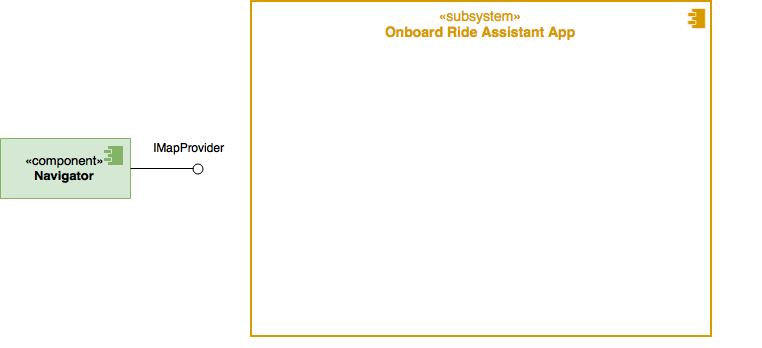
\includegraphics[scale=0.4]{{Figures/Integration/Integration0Car.png}}
    \caption{ORAA initial state}
    \label{fig:ORAA0}
    %TEXT
\end{figure}
As said in the previous section, the first component to be tested is Map Wrapper, since it requires only the IMapProvider interface provided by Navigator. IBookingProvider interface is shown since ClientAPI/Booking is being tested at this time. See \textit{Figure 2}.\\
\begin{figure}[h!]
    \centering
    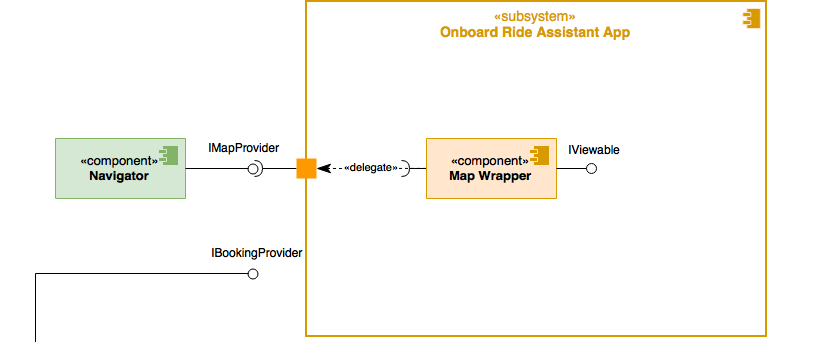
\includegraphics[scale=0.4]{{Figures/Integration/Integration1Car.png}}
    \caption{ORAA phase one}
    \label{fig:ORAA1}
    %TEXT
\end{figure}
Now Status Monitor can be tested, since it relies on the IBookingProvider interface that ClientAPI/Booking exposes. ClientAPI/Booking requires Booking Handler to answer queries, for the moment the stub used for ClientAPI/Booking testing will be in charge of providing the required data. See \textit{Figure 3}.\\
\begin{figure}[h!]
    \centering
    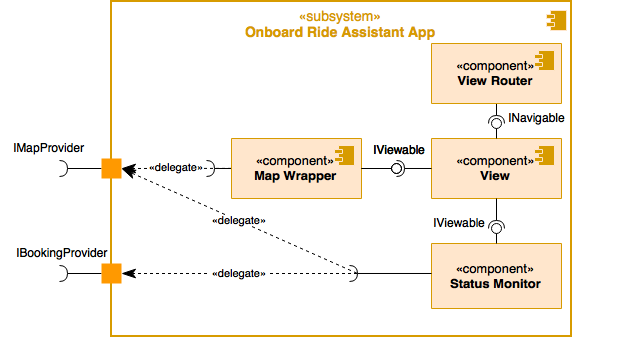
\includegraphics[scale=0.4]{{Figures/Integration/Integration2Car.png}}
    \caption{ORAA phase two}
    \label{fig:ORAA2}
    %TEXT
\end{figure}
Last components of the Onboard Ride Assistant App to be tested are View and View Router, whose testing will be carried out ensuring that all possible navigation paths established in the UX Diagram contained in the Design Document are possible, and the View always provide the right information with respect to UX Diagram and the Mockups in RASD. See \textit{Figure 3}.\\
\begin{figure}[h!]
    \centering
    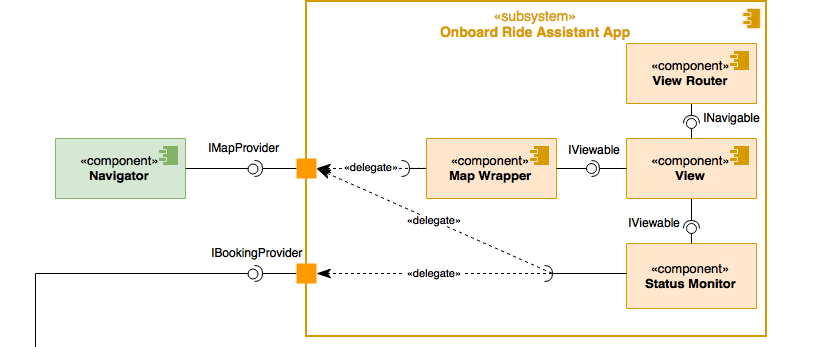
\includegraphics[scale=0.4]{{Figures/Integration/Integration3Car.png}}
    \caption{ORAA phase three}
    \label{fig:ORAA3}
    %TEXT
\end{figure}


\newpage
%SBL
\paragraph{Service Business Logic subsystem}
Service Business Logic subsystem needs to interact with a variety of third party systems most of which is already available since the beginning of testing. In particular Payment Processor Provider, Mail Server and Live Vehicle API are available for sure, while Entity Framework might still be under completion. See \textit{Figure 5}.\\
\begin{figure}[h!]
    \centering
    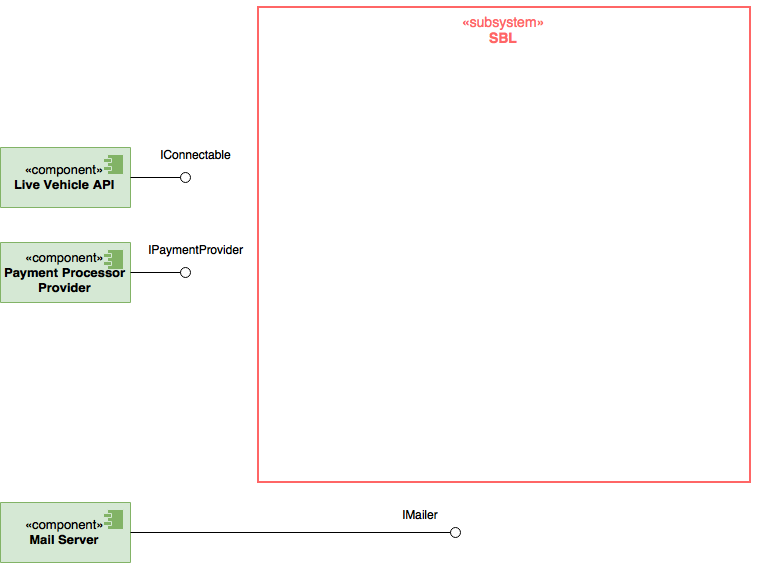
\includegraphics[scale=0.3]{{Figures/Integration/Integration0SBL.png}}
    \caption{SBL initial state}
    \label{fig:SBL0}
    %TEXT
\end{figure}
As said, Entity Framework might not be fully defined yet, in order to not delay PEJ Context testing we will use a stub if the Entity Framework is not already available. Otherwise the actual Entity Framework can be used. That's the reason way both Entity Framework and PEJ Context are shown in \textit{Figure 6}.\\
\begin{figure}[h!]
    \centering
    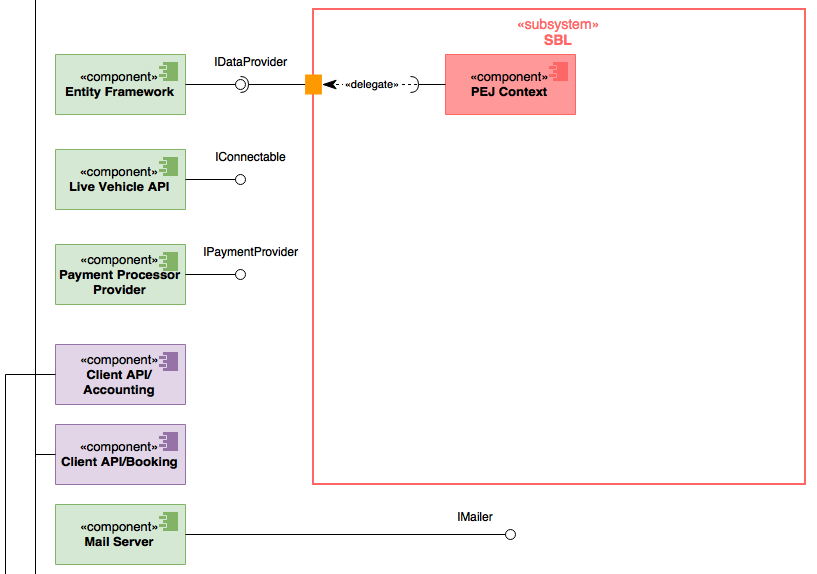
\includegraphics[scale=0.3]{{Figures/Integration/Integration1SBL.png}}
    \caption{SBL phase one}
    \label{fig:SBL1}
    %TEXT
\end{figure}
Moving on, four components can be tested at the same time: Special Areas Assistant and Vehicle Tracker, which requires a driver since Zone Manager is not tested, Payment Processor and Account Manager, which requires a driver since Booking Handler is not tested. Furthermore if Account Manager is tested before Account component in USMA, Account will be substituted by a driver, otherwise the actual Account component can be used in testing Account Manager. See \textit{Figure 7}.\\
\begin{figure}[h!]
    \centering
    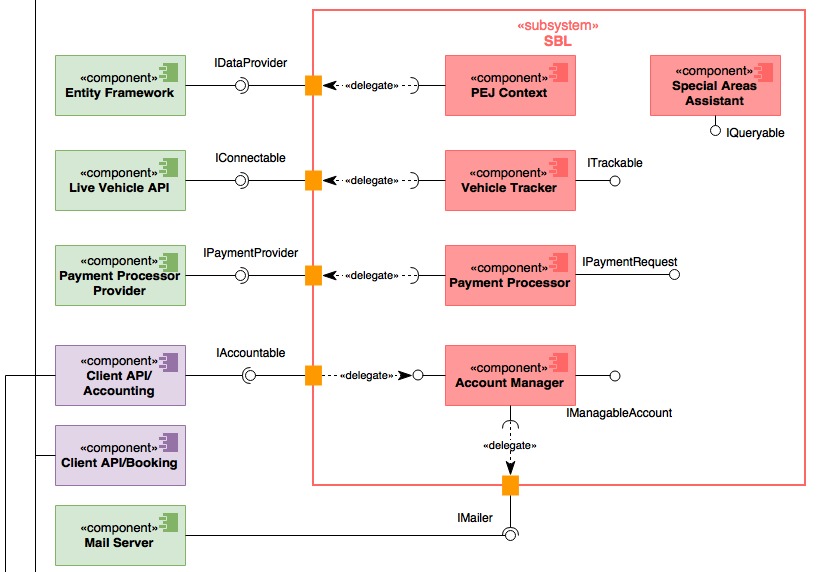
\includegraphics[scale=0.3]{{Figures/Integration/Integration2SBL.png}}
    \caption{SBL phase two}
    \label{fig:SBL2}
    %TEXT
\end{figure}
Zone Manager is tested, except for Booking Handler, all other components are now tested; this way Zone Manager doesn't need any stub and can be tested using just one driver instead of the actual Booking Handler. See \textit{Figure 8}.\\
\begin{figure}[h!]
    \centering
    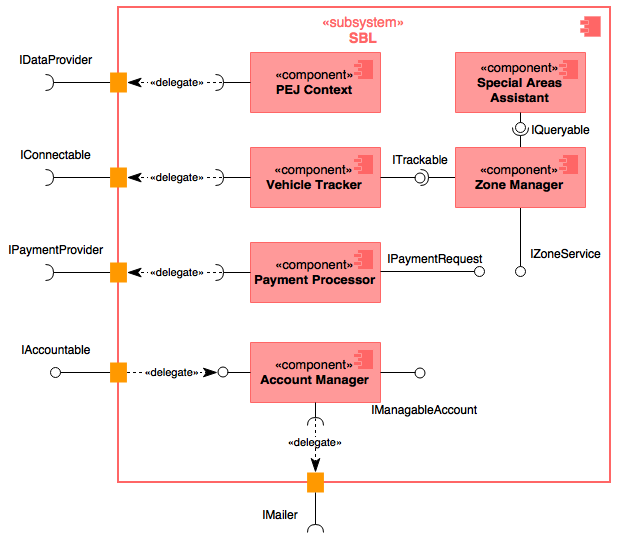
\includegraphics[scale=0.3]{{Figures/Integration/Integration3SBL.png}}
    \caption{SBL phase three}
    \label{fig:SBL3}
    %TEXT
\end{figure}
All other components are tested, so Booking Manager can now be tested without the need for any stub or driver. See \textit{Figure 9}.\\
\begin{figure}[h!]
    \centering
    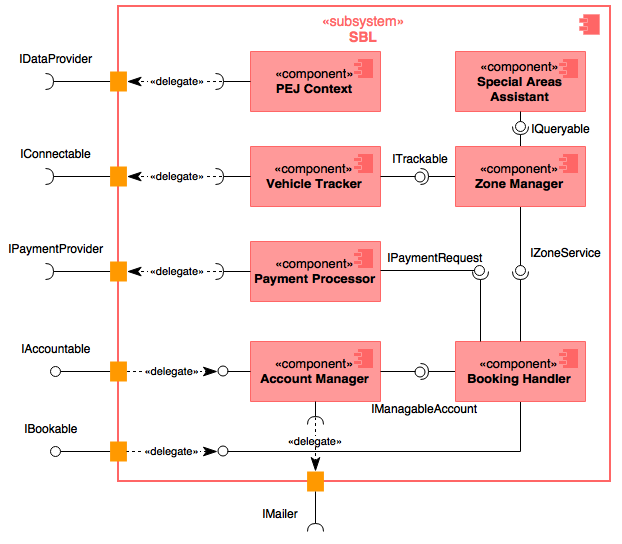
\includegraphics[scale=0.3]{{Figures/Integration/Integration4SBL.png}}
    \caption{SBL phase four}
    \label{fig:SBL4}
    %TEXT
\end{figure}

\newpage
%UDMA
\paragraph{User Device Mobile App subsystem}
As said before, Google Maps is already available, thus the initial situation is the one shown in the \textit{Figure 10}.\\
\begin{figure}[h!]
    \centering
    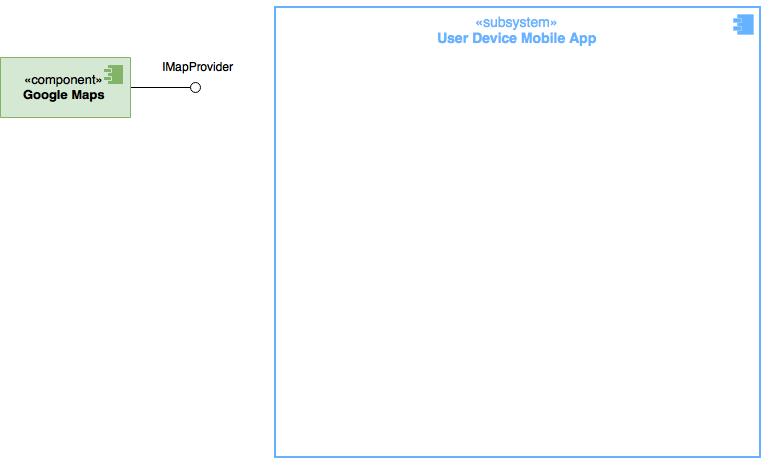
\includegraphics[scale=0.3]{{Figures/Integration/Integration0Mobile.png}}
    \caption{UDMA initial state}
    \label{fig:UDMA0}
    %TEXT
\end{figure}
The first component to the testes is the Map Wrapper. IBookingProvider and IAccounting Provider interfaces are shown since both ClientAPI are being tested at this time. See \textit{Figure 11}.\\
\begin{figure}[h!]
    \centering
    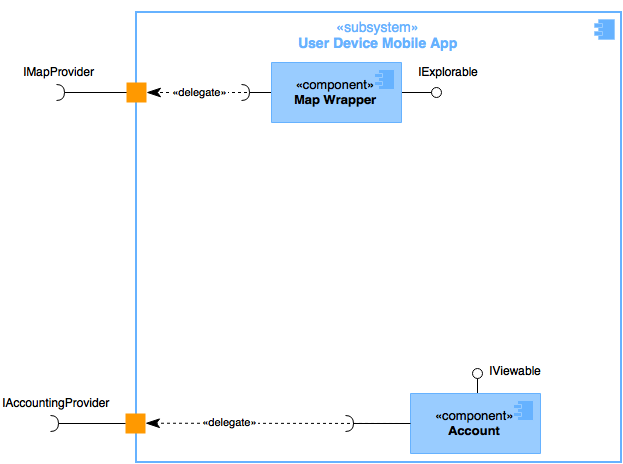
\includegraphics[scale=0.3]{{Figures/Integration/Integration1Mobile.png}}
    \caption{UDMA phase one}
    \label{fig:UDMA1}
    %TEXT
\end{figure}
Next are Map Explorer, Reserved Car Viewer and Account. The latter is tested relying on the data provided by Account Manager if it is already tested, or by the stub of ClientAPI/Accounting, while the first the component of the list require ClientAPI/Booking, which must rely on its stub since Booking Handler is the last component to be tested. See \textit{Figure 12}.\\
\begin{figure}[h!]
    \centering
    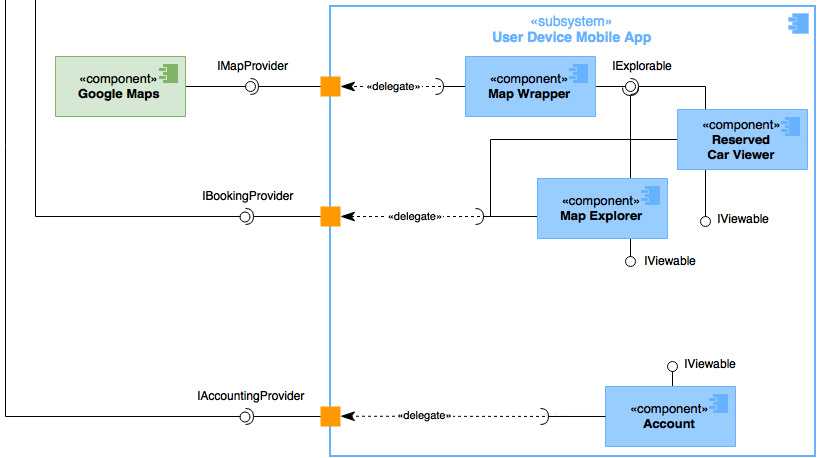
\includegraphics[scale=0.3]{{Figures/Integration/Integration2Mobile.png}}
    \caption{UDMA phase two}
    \label{fig:UDMA2}
    %TEXT
\end{figure}
Lastly View and View Router, whose testing will be carried out ensuring that all possible navigation paths established in the UX Diagram contained in the Design Document are possible, and the View always provide the right information with respect to UX Diagram and the Mockups in RASD. See \textit{Figure 13}.\\
\begin{figure}[h!]
    \centering
    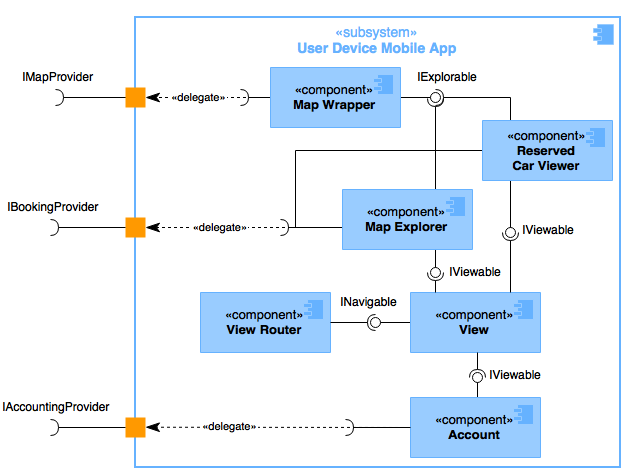
\includegraphics[scale=0.3]{{Figures/Integration/Integration3Mobile.png}}
    \caption{UDMA phase three}
    \label{fig:UDMA3}
    %TEXT
\end{figure}


\newpage
\subsubsection{Subsystem Integration Sequence}
After the single subsystems have been tested it it possible to integrate them. The last subsystem to be tested is SBL, which means that by the time it is tested the other two subystems will already be tested. This means the integration sequence can start either from ORAA or from UDMA by inegrating it with the SBL, to conclude with the intrgration of the other subsystem with system reulted from the previous integration. The final result can be seen in \textit{Figure 14}.
\begin{figure}[h!]
    \centering
    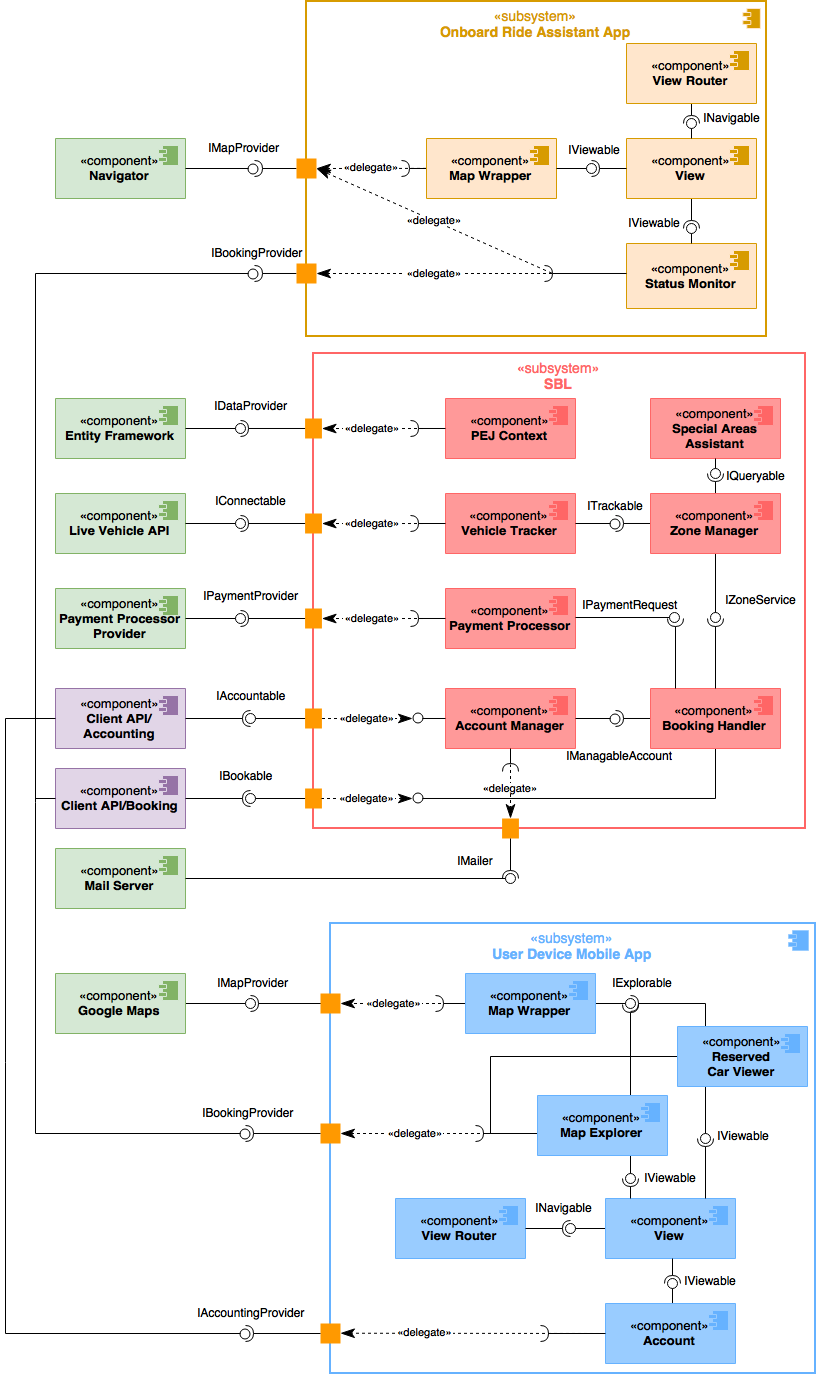
\includegraphics[scale=0.3]{{Figures/Integration/IntegrationFULL.png}}
    \caption{integrated subsystems}
    \label{fig:FULL}
    %TEXT
\end{figure}